%Om filen typsätts som del av hela rapporten så finns \master definierat i början och ingen \begin{document} och \end{document} får finnas, men för att kunna typsätta filen för sig är dem ett måste! \newcommand{\master}{} krävs i början på huvudrapporten!
\ifdefined\master
\else
	\documentclass[twocolumn]{article}
	\usepackage{graphicx}
	\usepackage{float}
	\usepackage{alltt}
	\begin{document}
\fi

\subsection{Outputs}
Two methods of gathering output data are available

\subsubsection*{Oscilloscope}
The oscilloscope has two functions, picture and measurement. The picture option practicaly takes a copy of the oscilloscope screen and shows it in the panel. The measurement option is used for getting the graph and plot it without all extra information the oscilloscope shows. The plot is then displayed in the panel. After entering the \emph{GPIB address} for the oscilloscope, the \emph{Start} button will execute the option chosen. (Fig. \ref{fig:osc})

\begin{figure}[H]
\centering
\fbox{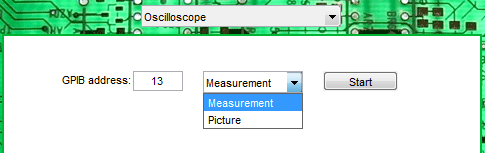
\includegraphics[width=6cm]{Figure/out_oscilloscope.png}}
\caption{Oscilloscope output settings.}
\label{fig:osc}
\end{figure}

\subsubsection*{Multimeter}
The multimeter function is just a multimeter, that displays the value in the panel. It's not possible to store the value as it is with a picture.  (Fig. \ref{fig:multi})

\begin{figure}[H]
\centering
\fbox{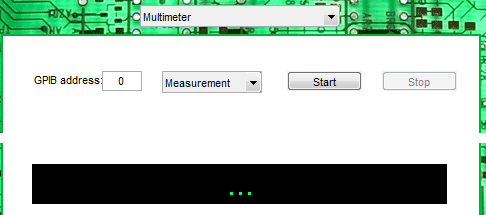
\includegraphics[width=7cm]{Figure/Multimeter.png}}
\caption{Multimeter output settings.}
\label{fig:multi}
\end{figure}

\subsubsection*{Bode Graph}
When the frequency sweep is chosen in the input panel it automaticaly chose the bode graph in the output panel. The Bode Graph only works with the frequency sweep as the start button is placed in the input panel. The plot is shown in the output panel. (Fig. \ref{fig:bode})

\begin{figure}[H]
\centering
\fbox{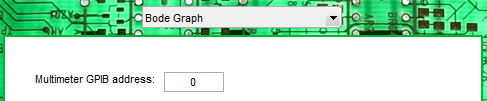
\includegraphics[width=6cm]{Figure/bode_graph.png}}
\caption{Bode plot output settings.}
\label{fig:bode}
\end{figure}


\ifdefined\master
\else
	\end{document}
\fi